% This file provides an example Beamer presentation using the RWTH theme
% showcasing some of the more common options, similar to the Powerpoint version
% 12.11.2014: Revision 1 (Harold Bruintjes, Tim Lange)

% For RWTH, beamer should be loaded with class option t (top)
\documentclass[t]{beamer}

% Use fontspec to get Arial font
% Requires use of XeLaTeX
\usepackage{fontspec}
\setmainfont{Arial}
\setsansfont{Arial}
% Also force Arial for math for a more consistent look
\usepackage{unicode-math}

% German style date formatting (footer)
\usepackage[ddmmyyyy]{datetime}
\renewcommand{\dateseparator}{.}

\usepackage{MnSymbol,wasysym}

% Format the captions used for figures etc.
\usepackage[compatibility=false]{caption}
\captionsetup{singlelinecheck=off,justification=raggedleft,labelformat=empty,labelsep=none}

% PGFPlots is used for drawing some of the charts
\usepackage{pgfplots}
\pgfplotsset{compat=newest}
% This file contains some styles and macros for drawing charts similar to those of MS Office

\pgfplotsset{hor_barchart/.style={
  xbar=0mm,
  xmin=0,
  xtick=\empty,
  axis y line*=left,
  x axis line style={opacity=0},
  bar width=0.6cm,
  ytick=data,
  nodes near coords,
  every axis/.append style={font=\normalsize},
  every node near coord/.append style={font=\normalsize},
  nodes near coords align={horizontal},
  legend style={at={(0,-10mm)},anchor=north west,legend columns=-1,draw=none},
}}

\pgfplotsset{ver_barchart/.style={
  ybar=0mm,
  x = 4.5cm,
  ymin=0,
  ymajorgrids,
  axis x line*=bottom,
  y axis line style={opacity=0},
  bar width=0.8cm,
  enlarge x limits={0.15},
  xtick=data,
  nodes near coords,
  every axis/.append style={font=\normalsize},
  every node near coord/.append style={font=\normalsize},
  nodes near coords align={vertical},
  legend style={at={(0,-10mm)},anchor=north west,legend columns=-1,draw=none},
}}

\tikzstyle{chart}=[
    legend label/.style={font={\normalsize},anchor=west,align=left},
    legend box/.style={rectangle, draw=none, minimum size=5pt},
]

\tikzstyle{pie chart}=[
    chart,
    slice/.style={line cap=round, line join=round,draw=none},
    pie title/.style={font={\bf}},
    slice type/.style 2 args={
        ##1/.style={fill=##2},
        values of ##1/.style={}
    }
]

\newcommand{\pie}[3][]{
    \begin{scope}[#1]
    \pgfmathsetmacro{\curA}{90}
    \pgfmathsetmacro{\r}{1}
    \def\c{(0,0)}
    \node[pie title] at (90:1.3) {#2};
    \foreach \v/\s in{#3}{
        \pgfmathsetmacro{\deltaA}{\v/100*360}
        \pgfmathsetmacro{\nextA}{\curA + \deltaA}
        \pgfmathsetmacro{\midA}{(\curA+\nextA)/2}

        \path[slice,\s] \c
            -- +(\curA:\r)
            arc (\curA:\nextA:\r)
            -- cycle;

        %\begin{pgfonlayer}{foreground}
        % Position labels at 1.2 times radius (just outside of chart)
        \path \c -- node[pos=1.2,pie values,values of \s]{$\v\%$} +(\midA:\r);
        %\end{pgfonlayer}

        \global\let\curA\nextA
    }
    \end{scope}
}

% Custom legend (used for pie chart)
\newcommand{\legend}[2][]{
\begin{scope}[#1]
  \path
    \foreach \n/\s in {#2} {
      ++(0,-5pt) node[\s,legend box] {} +(5pt,0) node[legend label] {\n}
    };
\end{scope}
}



%custom
\usepackage{tikz}
\usetikzlibrary{trees}
\usetikzlibrary{automata, positioning}
\usepackage{listings}
\lstset{basicstyle=\ttfamily}
\usepackage{tcolorbox}
\usepackage{framed}
\usepackage{forest}
\usepackage{xcolor}
\usepackage{blkarray}
\usepackage{comment}

% Define C++ style
\lstdefinestyle{cppStyle}{
    language=C++,
    basicstyle=\Large\ttfamily,
    keywordstyle=\color{blue},
    stringstyle=\color{purple},
    commentstyle=\color{green!60!black},
    morecomment=[l][\color{magenta}]{\#},
    tabsize=2,
    breaklines=true,
    showtabs=false,
    showspaces=false,
    showstringspaces=false,
    columns=flexible
}

\lstdefinestyle{antlr}{
    language=Java,
    morekeywords={grammar,returns},
    keywordstyle=\\color{blue},
    basicstyle=\ttfamily,
    tabsize=2,
    breaklines=true,
    showtabs=false,
    showspaces=false,
    showstringspaces=false,
    columns=flexible
}


\renewcommand{\Coloneqq}{\mathrel{\mathop{::}}=}
\newcommand*{\mybox}[1]{\framebox{#1}}

\setbeamertemplate{bibliography item}{\insertbiblabel}

% Load the actual RWTH theme. Suggested is to load the full theme,
% as it requires some specific dimensions
\usetheme{rwth}

\begin{document}

    \logo{
\includegraphics{logo}}

% Setup presentation information
    \title{Syntaktische Mehrdeutigkeiten \\ Erkennung, Vermeidung und Auflösung}
    \date{14.06.2024}
    \author{Lennart Protte}

    \frame{\titlepage}


    \section{Motivation}\label{sec:motivation}
    \begin{frame}
        \vspace{1em}
        \begin{columns}[T]
            \column{0.5\textwidth}
            \centering
            \begin{block}{Zielsetzung}
                \vspace{1em}
                Entwicklung von Strategien zur \textbf{Erkennung} und \textbf{Lösung} von Mehrdeutigkeiten
                oder zur \textbf{Vermeidung} ihrer Entstehung.
                \vspace{1em}
            \end{block}
            \column{0.5\textwidth}
            \centering
            \begin{tikzpicture}[node distance=1.5cm, auto, every node/.style={align=center}]
                % Nodes
                \node (avoid) [rectangle, draw, left of=input, text centered, minimum height=1cm, minimum width=2.5cm, xshift=-4.5cm] {Vermeidung};
                \node (input) [rectangle, draw, text centered, minimum height=1cm, minimum width=2.5cm] {Mehrdeutigkeiten};
                \node (detect) [rectangle, draw, below of=input, text centered, minimum height=1cm, minimum width=2.5cm, yshift=-0.5cm] {Erkennung};
                \node (solve) [rectangle, draw, below of=detect, text centered, minimum height=1cm, minimum width=2.5cm, yshift=-0.5cm] {Lösung};

                % Arrows
                \draw[->] (input) -- (avoid);
                \draw[->] (input) -- (detect);
                \draw[->] (detect) -- (solve);
            \end{tikzpicture}
        \end{columns}
        \vspace{1em}
        \begin{exampleblock}{Beispiel}
            Manchmal lassen sich Mehrdeutigkeiten nicht vermeiden. \\
            Dann ist es notwendig diese zu Erkennen und Aufzulösen.
        \end{exampleblock}
    \end{frame}


    \section{Probleme und Herausforderungen}\label{sec:probleme-und-herausforderungen}
    \begin{frame}
        \begin{block}{Problemstellungen}
            \begin{itemize}
                \item Bei komplexen Programmiersprachen lassen sich Mehrdeutigkeiten kaum vermeiden.
                \item Es existiert kein Algorithmus, welcher eindeutig Mehrdeutigkeiten erkennen kann.
                \item Mehrdeutigkeiten können nur selten Algorithmisch aufgelöst werden.
            \end{itemize}
        \end{block}
    \end{frame}


    \section{Vermeidung von Mehrdeutigkeiten}\label{sec:vermeidung-von-mehrdeutigkeiten}
    \begin{frame}[fragile]
        \begin{block}{Design eindeutiger Programmiersprachen}
            \begin{itemize}
                \item Symbole
                \item Bezeichner
                \item Vorrangsregeln
                \item Assoziativität
            \end{itemize}
        \end{block}
        \begin{columns}[T,onlytextwidth]
            \column{0.45\textwidth}
            \begin{exampleblock}{Mehrdeutiger C++ Code}
                \hspace*{-3em}
                \begin{minipage}{\textwidth+3em}
                    \begin{lstlisting}[style=cppStyle,label={lst:lstlisting1}]
            class A {public: void func() {}};
            class B {public: void func() {}};
            class C: public A, public B {};
            int main() {
                C c;
                c.func();
                return 0;
            }
                    \end{lstlisting}
                \end{minipage}
            \end{exampleblock}
            \column{0.48\textwidth}
            \begin{exampleblock}{Eindeutiger C++ Code}
                \hspace*{-3em}
                \begin{minipage}{\textwidth+3em}
                    \begin{lstlisting}[style=cppStyle,label={lst:lstlisting2}]
            class A {public: void func() {}};
            class B {public: void func() {}};
            class C: public A, public B {};
            int main() {
                C c;
                c.A::func();
                return 0;
            }
                    \end{lstlisting}
                \end{minipage}
            \end{exampleblock}
        \end{columns}
    \end{frame}


    \section{Erkennung von Mehrdeutigkeiten}\label{sec:erkennung-von-mehrdeutigkeiten}
    \begin{frame}
        \begin{block}{Methoden zur Erkennung von Mehrdeutigkeiten}
            \begin{itemize}
                \item Suchbasierte Mehrdeutigkeitserkennung
                \item Analyse der Parsing-Tabelle
                \item Analyze der Grammatik
            \end{itemize}
        \end{block}
        \begin{exampleblock}{Suchbasierte Merhdeutigkeitserkennung}
            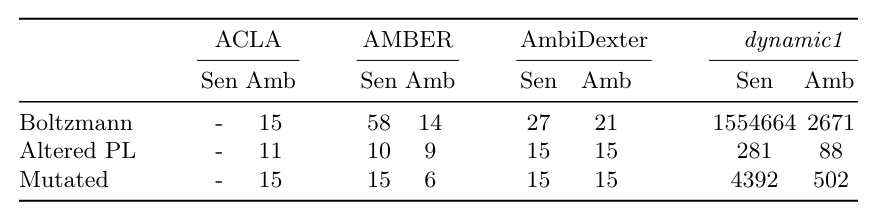
\includegraphics[width=\textwidth]{./detectors}\cite{springer2013}
        \end{exampleblock}
    \end{frame}


	\section{Auflösung von Mehrdeutigkeiten}\label{sec:auflsung-von-mehrdeutigkeiten}
	\begin{frame}
		\begin{columns}[T]
			\column{0.45\textwidth}
			\begin{block}{Chomsly Normalform}
				Für $A,B,C \in N$, $S \in \text{Startsymbol}$, $a \in T$ und $B,C \neq S$. \\
				\begin{align*}
					& A \rightarrow BC \\
					& A \rightarrow a \\
					& S \rightarrow \varepsilon
				\end{align*}
			\end{block}
			\begin{exampleblock}
				\begin{itemize}
					\item Mehrdeutigkeiten können durch die Umformung in eine CNF aufgelöst werden.\cite{kemp1974}
					\item Vereinfacht es eine weitere Analyse der Grammatik.
				\end{itemize}
			\end{exampleblock}
			\column{0.45\textwidth}
			\begin{block}{Algorithmus von Vasudevan und Tratt}
				\begin{align*}
					& E \Coloneqq E * E \phantom{|} & (links) \\
					& > E + E & (links) \\
					& \phantom{|} | \phantom{|} \bold{num}
				\end{align*}
			\end{block}
			\begin{exampleblock}
				Kann unter gegebener Assotiativität und Vorrangsregeln eine eindeutige Grammatik erzeugen.

			\end{exampleblock}
		\end{columns}
	\end{frame}


    \section{Praktische Ansätze}\label{sec:praktische-ansatze}
    \begin{frame}[fragile]
        \begin{block}{ANTLR}
	        \hspace*{-3.5em}
            \begin{minipage}{\textwidth+3.5em}
                \begin{lstlisting}[style=antlr,label={lst:lstlisting3}]
        start   : statement* EOF ;
        statement: 'if' condition 'then' statement ('else' statement)?? ;

        condition: '(' STRING ')' ;
        STRING   : '"' .*? '"' ;
        WS       : [ \t\r\n]+ -> skip ;
                \end{lstlisting}
            \end{minipage}
        \end{block}
        \vspace{1em}
        \begin{exampleblock}{Erläuterung des \(??\) Operators}
            Der \(??\) Operator gibt dem Else die niedrigste Priorität, womit es mit dem äußersten If gematched wird. \\
        \end{exampleblock}\cite{parr}
    \end{frame}


    \section{Ausblick}\label{sec:ausblick-und-zukunftige-projekte}
    \begin{frame}
        \begin{itemize}
            \item Maschinelles Lernen zur Erkennung von Mehrdeutigkeiten
            \item Natürliche Sprache => Komplexe Mehrdeutige Grammatiken
        \end{itemize}
    \end{frame}


    \section{Quellen}\label{sec:quellen}
    \begin{frame}[allowframebreaks]
        \bibliographystyle{apalike}
        \bibliography{refs}
    \end{frame}

\end{document}